\newpage
\subsection{Caso d'uso UC9: Interazione con API Acquistate}
\label{UC9}
\begin{figure}[ht]
	\centering
	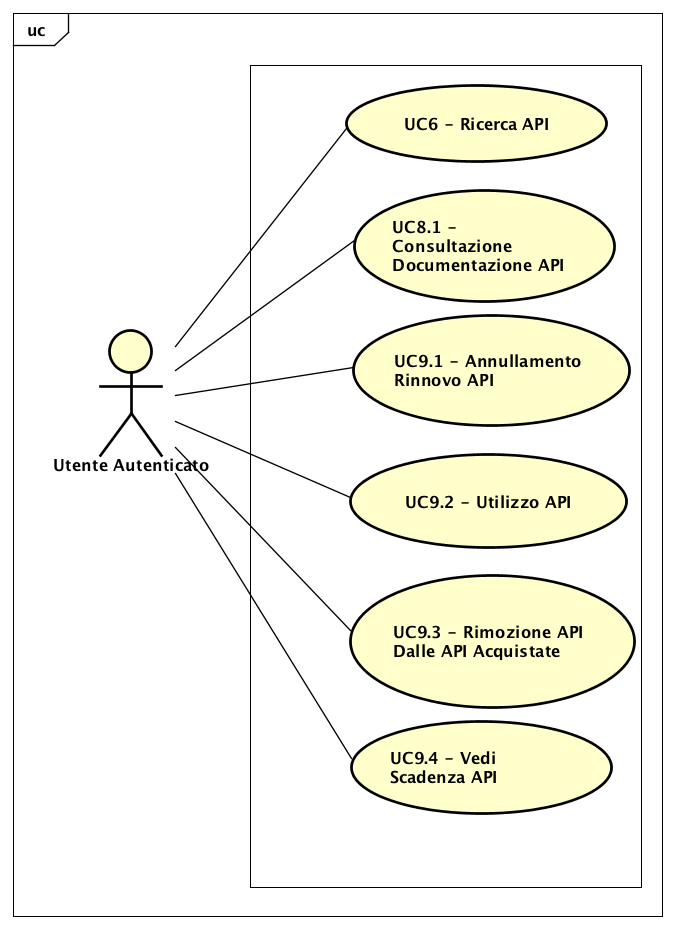
\includegraphics[scale=0.45]{UML/UC9.png}
	\caption{UC9: Interazione con API Acquistate}
\end{figure}
\FloatBarrier
\renewcommand*{\arraystretch}{1.6}
\begin{longtable}{ l | p{11cm}}
	\hline
	\rowcolor{Gray}
	\multicolumn{2}{c}{UC9: Interazione con API Acquistate} \\
	\hline
	\textbf{Attori} &Utente Autenticato, Amministratore APIMarket, Interfacce API Presente In APIMarket \\
	\textbf{Descrizione} & l'attore sceglie attraverso quale modalità interagire con le API acquistate \\
	\textbf{Pre-Condizioni} & l'attore si trova nella schermata di gestione di una API acquistata\\
	\textbf{Post-Condizioni}&l'attore ha scelto l'interazione\\
	\textbf{Scenario Principale} & \begin{enumerate*}[label=(\arabic*.),itemjoin={\newline}]
		\item L'attore può ricercare un'API(UC6)
		\item L'attore può consultare la documentazione di un'API(UC8.1)
		\item L'attore può Annullare il rinnovo di un'API(UC9.1)
		\item L'attore può utilizzare un'API(UC9.2)
		\item L'attore può Rimuovere un'API dalle Acquistate
		\item L'attore può vedere la Scadenza di un'API(UC9.4);
	\end{enumerate*}\\
\end{longtable}


